\documentclass{article}

% AMS math symbols
\usepackage{amsfonts}
\usepackage{amsmath}
\usepackage{amssymb}

% colored textare that buyers
\usepackage{color}

% Evolutional algorithms journal template
\usepackage{ecj}

% custom enumerates
\usepackage{enumitem}

% eps figures
\usepackage[pdftex]{graphicx}

% boxed figures
\usepackage{float}

% set page margins
\usepackage[top=1in, bottom=1in, left=1in, right=1in]{geometry}

% citations with author
\usepackage{natbib}

% additional colors
\usepackage[usenames,dvipsnames]{xcolor}

\newcommand{\concat}{\ensuremath{+\!\!\!\!+\,}}
\newcommand{\usman}{\textcolor{Red}{\textbf{*** USMAN ***} }}
\newcommand{\claudio}{\textcolor{Cerulean}{\textbf{*** CLAUDIO ***} }}

%\floatstyle{boxed} 
%\restylefloat{figure}

\setlength{\parskip}{7pt}
\setlength{\parsep}{0pt}
\setlength{\parindent}{0pt}

\setlist{nolistsep}

% ADDING A FIGURE
%\begin{figure}[t]
%\begin{center}
%\psfig{file=Bsimilar.eps,width=300pt}
%\end{center}
%\caption{NKY algorithm: performance of different implementations.}
%\label{fig:Bsimilar}
%\end{figure}
%

% CITING
% \citep{citation}

\begin{document}

% uncomment this to get journal footers
%\ecjHeader{x}{x}{xxx-xxx}{200X}{genetic vs deterministic algorithms for LCS}{C. A. Andreoni, U. Masood}
\title{Caching Fractal B+ Trees}

\author{\name{\bf Claudio Alberto Andreoni} \hfill \addr{caa@mit.edu}\\ 
        \addr{Department of Mathematics, Massachusetts Institute of Technology, 
        Cambridge, 02139, United States}
\AND
       \name{\bf Usman Masood} \hfill \addr{usmanm@mit.edu}\\
        \addr{Department of Electrical Engineering and Computer Science, Massachusetts Institute of Technology, 
        Cambridge, 02139, United States}
}

\maketitle

\begin{abstract}
The two primary requirements for database systems are handling data queries rapidly and utilizing storage thriftily.
However, these often stand in contrast with each other,
as traditionally space usage and achievable performance are inversely proportional.
In order to quickly retrieve data,
databases maintain an index of searchable keys, along with the location of the corresponding data on drive.
Modern systems such as IBM DB2, Oracle, and MS SQL Server use B+ trees for the indexes,
due to their ability to efficiently exploit disk bandwidth \citep{Gehrke:2002}.

Fractal B+ trees (FB+ trees), a kind of recursive B+ tree structure, were proposed to improve performance
by adapting to both disk layout and processor cache.
However, these either increase the amount of space wasted in representing the index,
or require an aggressive memory management scheme \citep{Chen:2002}.

We propose a new data structure named Caching Fractal B+ trees (CFB+ trees), which replicates the structure
of FB+ trees, but takes advantage of the wasted space to perform online caching of database entries.
CFB+ trees simplify the complexity associated with performing index operations,
and reduce in expectation the number of reads from disk necessary to retrieve the queried data. 
\end{abstract}

\section{Introduction}

\usman
\begin{enumerate}
	\item Give background on database systems and their needs (bottleneck of page reads)
	\item Operations needed, why B+ trees and not other structures
	\item Survey very briefly basics of B+ trees, page performance
	\item State that we're going to improve cache performance with the idea from the paper and then improve even further
caching tuples
\end{enumerate}

One of the key aspects of data design is that resources, especially disk bandwidth and memory, must be utilized efficiently. To utilize memory efficiently, databases cache \textit{hot} tuples in memory so that when querying for them, they can be fetched directly from memory rather than having to go to the disk. To utilize disk bandwidth efficiently, databases try to minimze the amount of disk pages read and perform sequential access to disk when possible. Disks are usually an order of magnitude slower than memory, and since data in databases needs to be persistent stored on disk, disk bandwidth tends to be the bottleneck for practically all workload.

To that end, databases often employ index structures over certain \textit{columns} to store tuple pointers so that they can be looked up in a way faster than scanning the entire relation. As long as the cost of reading the entire relation is less than the cost of searching for an item in the index structure and fetching a single tuple from disk, we should expect a performance improvement. In practice, all relations are large enough that index structures are helpful rather than detrimental to performance.

The way these index structures are used is that while adding a tuple we insert an entry to the index structure with the \textit{key} as the contents of the column we are indexing over, and the \textit{value} as the pointer to the on-disk location of the tuple. When retrieving a tuple, we search for the tuple in the index structure and use the pointer returned by it to read the tuple from disk. 

\subsection{B+ tree Indexes}
The index structure should provide operations such as insertion, deletion, search and in most cases range scan. B+ trees are a natural choice for index structures because they provide all the required operations and they can be optimized to exploit disk bandwidth efficiently. Some times hash tables are also used to index data, but since they do not support range queries they can only be used to index columns over which range queries are never performed. Lately, cache-oblivious Fractal Trees have also been employed as index structures.


\subsubsection{Optimizing B+ trees for Disk Performance}

To optimize I/O performance, traditional \textit{disk optimized} B+ trees are composed of nodes the size equal to a \textit{disk page} -- the natural transfer size for reading and writing to disk. Having such large nodes, means that the branching factor is usually quite large, on the order of hundreds. Having such a large branching factor means that the height of the tree is quite small. This is beneficial because only a few pages need to be read from disk inorder to find the tuple pointer we're looking for. At the same time, however, this also means that the additional page access to retrieve the associated tuple data is a significant part of the total cost. Typical index fill factors have been shown to be around 68\%, which is a concious decision to ensure that in the presense of inserts we do not have too many expensive node split operations. A major contribution of this paper is providing a scheme to utilize this wasted space as a tuple cache, so that for \textit{hot} tuples we can read the data directly from the leaf node page and avoid the additional disk page access we talked about earlier needed to reading tuple data.

Another downside of using traditional \textit{disk optimized} B+ trees is that they have poor cache performance. They incur an excessive number of cache misses, wasting time and forcing the eviction of useful data from the cache in the process. This is because of the large the discrepancy in node sizes and width of cache lines -- the natural size of reading and writing to main memory. A single cache line is usually 32B-128B wide and so the \textit{jumps} in a 4KB address space while binary searching a node are result in a lot of cache misses. Cache prefetching is helpful only when the range of the binary search becomes considerably small.

\subsubsection{Optimizing B+ trees for Cache Performance}

Recently, many studies have presented new typles of B+ trees -- \textit{cache-sensitive B+ trees}, \textit{prefetching B+ trees} -- optimized for cache performance. These datastructures try to minimize the impact of cache misses by making node sizes equal to to the width of a cache line (or some small multiple of it). However, this technique for cache optimization is at odds with disk performance. Small nodes result in a small branching factor, which means in searching from the root to the desired leaf, we might suffer a disk page access for each node on this path.

Fractal Prefetching B+ trees (fpB+ trees) are a type of B+ tree which try to optimize both disk and cache performance. In this paper, we propose Caching Fractal B+ trees (cfB+ trees) which extend fpB+ trees to improve cache performance further while ensuring comparable disk performance.

\section{Fractal B+ trees}
\usman
\begin{enumerate}
	\item Explain the data structure (don't go into SPLIT and MERGE though, I need to talk about these later)
	\item Say that the way they are used is index adn then you have to access the disk separately later 
	\item Give rationale for usage: have best disk performance, want to improve cache performance
	\item Add all your interesting observations about the relationship between parameters (bfactor etc etc)
\end{enumerate}
\claudio
Will make graphs if necessary to explain something

\section{Adding Caching: CFB+ trees}
\claudio
\subsection{Using Gaps for Good}
This far, we have illustrated how FB+ trees store a small B+ tree in each big node.
The strategy proposed for FB+ trees is to fragment big nodes into smaller nodes when the small trees
are mostly empty, and pack multiple big nodes in the same disk page.
Instead, when big nodes grow, the inverse strategy is applied and big nodes are split and spread
across pages.

This process adds complexity to the implementation, and only guarantees that pages are filled
homogeneously, not that space waste is minimized.
Indeed, when a big block the size of a page is split in half,
we can expect the former page to become half empty and the new one to become half full.

We propose instead that a page always represent a single big node, and the space gaps in the page
be exploited to cache database tuples.
Compared to the strategy for FB+ trees, we avoid compressing big nodes, resulting in an
even less efficient tree space usage.
However, we also exploit all the space which is not allocated to the tree to store cached tuples,
so that almost no space is left unused.

This allows to return searched tuples which are in cache without the additional overhead of reading a page from
the actual tuple storage.
The operating system tries to maintain pages which are accessed frequently in memory for faster
access.
Also, pages belonging to the index are accessed more often than tuple pages, because every operation
needs to walk a path in the index.
Therefore, caching tuples in the index has the double advantage of reducing the likelihood
of a read to tuple page which is not in memory, and reducing the need for the operating systems
to replace index pages in memory with tuple pages.
The same fact remains relevant for integrated database systems, which strongly enforce the policy of keeping
index pages in memory.


\subsection{Patterns of Memory (Un)Usage}

We refer to the memory space necessary to store a small node as a \textit{slot}.
Each big node contains a fixed number $\sigma$ of slots, part of which will be in use
as small nodes, while the rest will be available for cache (Figure \ref{fig:inner_block}).
\begin{figure}[h]
\begin{center}
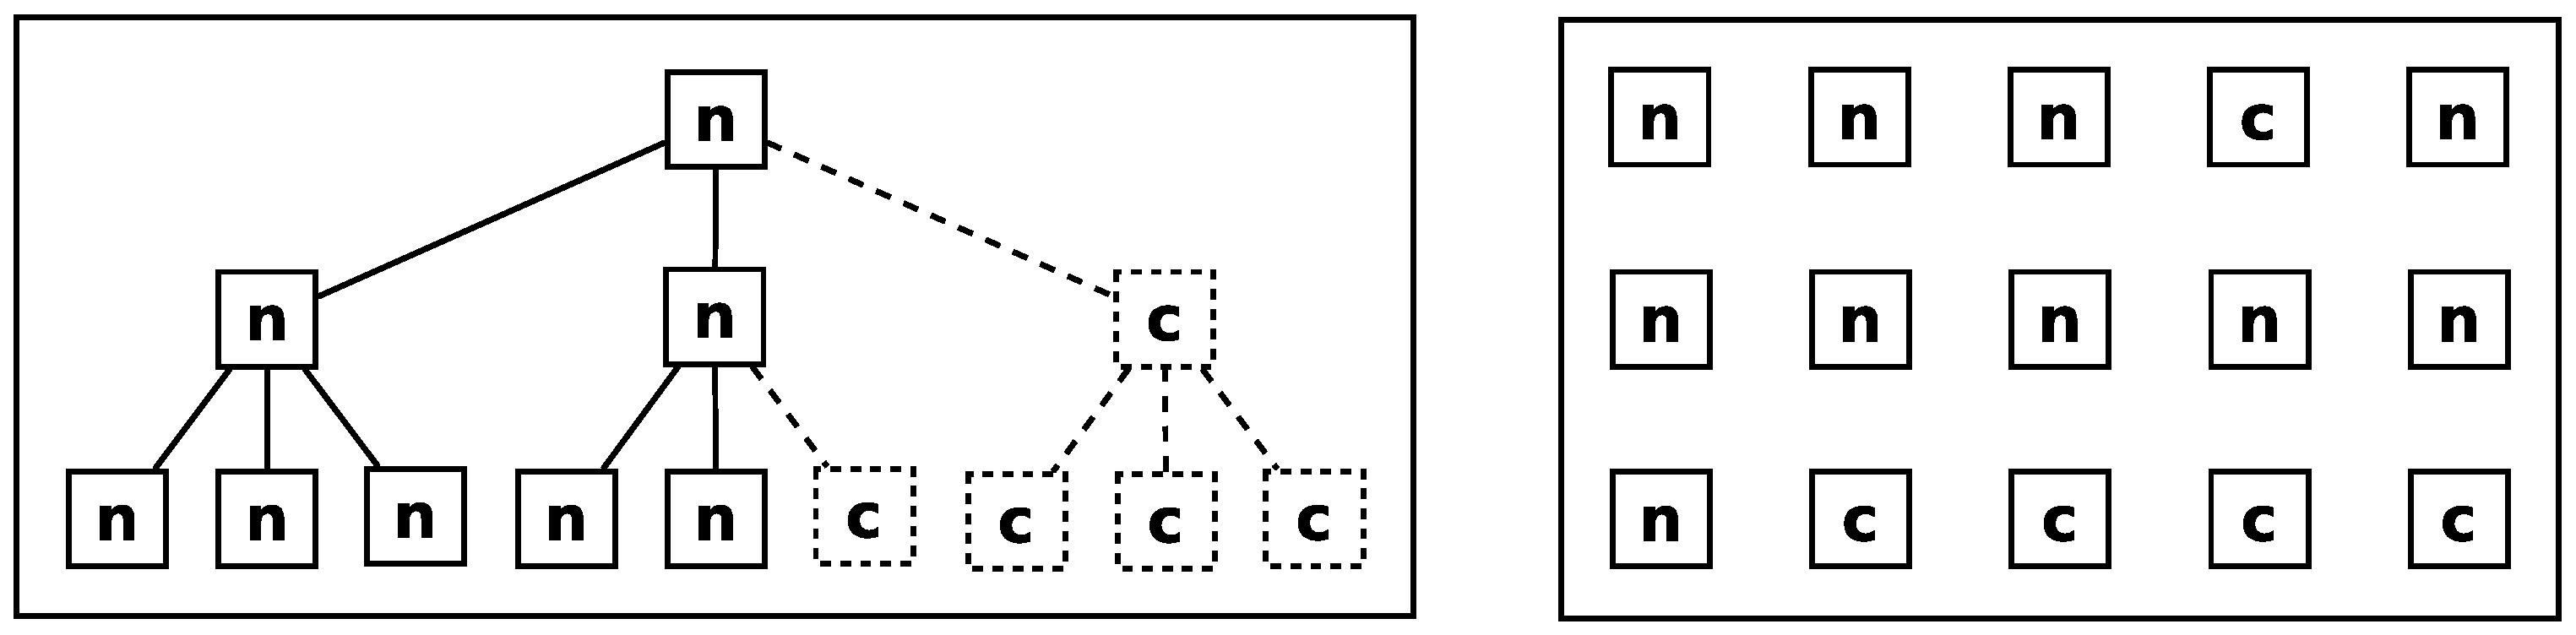
\includegraphics[width=350pt]{inner_block}
\end{center}
\caption{
The content of a big node.
On the left, a small tree as it is interpreted logically.
On the right, a small tree laid out in memory, with slots available for cache.
}
\label{fig:inner_block}
\end{figure}

In order to justify our choice to utilize unused slots as cache,
we remark that -- under standard database loads --
B+ trees tend to be full at around 60\% of their capacity \citep{Wu:2011}.
Thus, given that the tree should be fairly well balanced,
we expect to have $0.4 \sigma$ slots available for cache on average in leaf big blocks.
As long as tuples are small enough to fit in a single slot,
we expect then to be able to cache most of the tuples indexed in the tree.

Furthermore, unused slots are all the same size, and they are all located at an integer multiple
of the slot size, making them easy to access and fast to read without much overhead.


\subsection{Caching tuples}
An important fact to notice is that the pattern of insertions and removals determines the shape of the tree;
therefore, the distribution of slots available for cache in memory is hard to analyze.
Moreover, as items are inserted and removed, new nodes are also added and removed;
correspondingly, slots that were once available are allocated to the
tree and become unavailable to the cache, and vice-versa.
This is evident even from Figure \ref{fig:inner_block}, which illustrates that
slots available for cache are sparse in the big node.

It is apparent then that the scenario is reminescent of that of a hash table.
In fact, we can consider the function that allocates slots to the small tree to be an adversary
hash function taking away and releasing cache slots outside of the control of our cache system.
We can then interpret the problem as that of finding a suitable hash system to insert and retrieve
cache entries in unused slots.

Intuitively, a candidate hashing strategy can take inspiration from open addressing.
Conside a big node $B$ on the path to the leaf that points to tuple $\tau$.
With open addressing, we insert by repeatedly hashing the key for $\tau$ to a slot in $B$,
till we find a slot that is available for cache and has room for one more cache entry.
Similarly, we search by repeatedly hashing the key for $\tau$ till we either find
a cache slot containing $\tau$, we find a cache slot with room for more entries,
or we have probed every slot in the big node.
With this scheme, a cache slot converted to a tree node effectively results
in the cache entries at that slot being evicted from cache.

Notice that, unlike for the case of traditional open addressing, we do not assume an item is not cached
if we hash to a slot that has available room but does not contain it.
That is because otherwise, when a tree node is released and made available from cache, we would risk
invalidating parts of the cache.
In spite of the fact that we may need to probe all slots often, performance may not degrade in practice
thanks to prefetching.
Modern processors have L1D (data level-1 cache) in the order of tens of KB, so the entire big node
can be prefetched and loaded at negligible cost by precomputing the next slots to be probe and request
a prefetch.


how we do it \\
why open addressing (many holes so good perf), linear probing \\
why not other hashing (cuckoo/hopscotch better in theory, but we cannot displace nodes allocated to tree) \\


\section{Experimental Results}

\subsection{Implementations}
\claudio
Describe some details of the implementations \\
how we compress big nodes in amortized O(1)\\
we could use jump pointers to exploit prefetching for range queries (which we didn't consider) \citep{Chen:2001} \\
Complexity, why we didn't go for cache oblivious sizing (split stage would be a nightmare)

For all benchmarks in this paper, we use a system based on an Intel Core i7 920 with 4 GB of RAM.
All code was written in the C language, and compiled with gcc version 4.6.1.

\subsection{Benchmarks}
\usman
\begin{enumerate}
	\item Make benchmarks and collect all performance data
	\item Explain why the benchmarks are relevant / useful / interesting
\end{enumerate}
\claudio
Make plots after the data is collected


\section{Conclusions}
\claudio
Summarize and remark that we managed to improve.

\small

\bibliographystyle{apalike}
\bibliography{final}


\end{document}
